\icode{N24L-T-CA-L3-261011-001}
\nceeID{24山东}{16}
战国时期青铜汲酒器，根据其原理制作了由中空圆柱形长柄和储液罐组成的汲液器，如图所示。长柄顶部封闭，横截面积 \( S_1 = \)\,\qty{1.0}{cm^2}，长度 \( H =  \) \,\qty{100.0}{cm}，侧壁有一小孔 \(A\)。储液罐的横截面积 \( S_2 = \) \,\qty{90}{cm^2}，高度 \( h =  \) \,\qty{20.0}{cm}，罐底有一小孔 \(B\)。汲液时，将汲液器竖直浸入液体，液体从孔 \(B\) 进入，空气由孔 \(A\) 排出；当内外液面相平时，长柄浸入液面部分的长度为 \( x \)；堵住孔 \(A\)，缓慢地将汲液器竖直提出液面，储液罐内刚好装满液体。已知液体密度 \( \rho =  \) \,\qty{1.0e3}{kg\per m^3}，重力加速度大小 \( g =  \) \,\qty{10}{m\per s^2}，大气压 \( p_0 = \) \,\qty{1.0e5}{Pa}。整个过程温度保持不变，空气可视为理想气体，忽略器壁厚度。

\begin{enumerate}
    \item 求\(x\)；
    \item 松开孔\(A\)，从外界进入压强为\(p_0\)、体积为\(V\)的空气，使潢储液罐中液体缓慢流出，堵住孔\(A\)，稳定后罐中恰好剩余一半的液体，求\(V\)。
\end{enumerate}

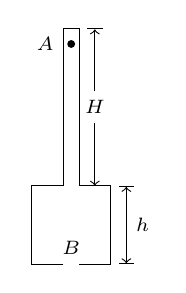
\begin{tikzpicture}[font=\scriptsize]
    \draw[|<->] (.3,3)--node[fill=white]{\(H\)}(.3,1);
    \draw (-.1,0)--(-.5,0)--(-.5,1)--(-.1,1)--(-.1,3)--(.1,3)--(.1,1)--(.5,1)--(.5,0)--(.1,0);
    \fill (0,2.8) circle(.05);
    \draw[|<->|] (.7,1)--node[right]{\(h\)}(.7,0);
    \node at(-.1,2.8)[left]{\(A\)};
    \node at(0,0)[above]{\(B\)};   
\end{tikzpicture}
\begin{answer}
    （1）\(x =\) \,\qty{2}{cm}（2）\(V =\)\, \qty{8.92e-4}{m^3}
\end{answer}